\documentclass[journal=jacsat,manuscript=article]{achemso}
\usepackage[version=3]{mhchem}
\usepackage[english]{babel}
\usepackage[utf8]{inputenc}
\usepackage{anysize}
\usepackage{float}
\usepackage{graphicx}
\usepackage{siunitx}
\usepackage{chemscheme}

% AUTHORS
\author{Cristina Ruiz}
\altaffiliation{Both authors have equally contributed}
\author{Álvaro Raya-Barón}
\altaffiliation{Both authors have equally contributed}
\author{Manuel A. Ortuño}
\affiliation[b]{Institute of Chemical Research of Catalonia (ICIQ), The Barcelona Institute of Science and Technology (BIST), Av. Països Catalans 16, 43007 Tarragona, Spain.}
\email{mortuno@iciq.es}
\author{Ignacio Fernández}
\email{ifernan@ual.es}
\affiliation[a]{Department of Chemistry and Physics, Research centre CIAIMBITAL, Ctra. Sacramento, s/n, 04120 Almería, Spain.}

%FALTAN LAS ABREVIATURAS Y PALABRAS CLAVE

% TITLE
\title{Accelerating role of deaggregation agents in lithium-catalysed hydrosilylation of carbonyl compounds} %Electronic supplementary information (ESI) available: Kinetic plots, NMR spectra, computational details, intermediate and transition state structures. See DOI: 10.1039/d0dt01540g

% MANUSCRIPT
\begin{document}
	\maketitle
	
	% ABSTRACT
	
	\begin{abstract}
		{\bf https://github.com/cristiruizblaze/proyecto\_final}
		\\
		A combined computational and experimental approach demonstrates the accelerating role of deaggregation agents, especially HMPA, in the Li-catalysed hydrosilylation of acetophenone in THF solution under very mild conditions.
	\end{abstract}
	
	% INTRODUCTION
	
	\section{Introduction}
	The reduction of carbonyl groups into alcohols is of wide interest in synthetic chemistry and therefore, constant efforts are	put into developing new efficient methodologies and perfecting the existing ones. Catalytic hydrosilylation\cite{Magnus1999} has emerged as a convenient method as it operates under mild conditions and combines an exceptional reducing capability with a high selectivity that can be finely tuned via catalyst design.
	
	% STATE OF THE ART
	
	\section{State of the art}
	Many Earth-abundant first-row transition metals, specially iron,\cite{Nishiyama2007,Tondreau2008,Yang2010,Raya-Baron2019} have been tested in catalytic hydrosilylation of carbonyl compounds, as they are usually more environmentally-friendly and less toxic than their second- and third-row counterparts. Alkali metal salts have also been explored as alternative catalysts, initially by the groups of Corriu\cite{Corriu1990} and Hosomi,\cite{Hosomi1986} and later by Beller\cite{Addis2010} and Nikonov\cite{Revunova2014} among others. Such compounds have been employed to promote hydrosilylation due to their basic character via formation of a pentacoordinated hydridosilicate, usually neglecting any relevant role of the alkali cation in the reaction mechanism. We recently reported	the hydrosilylation of carbonyl compounds catalysed by lithiated hydrazones. However, full understanding at atomic level of detail is still needed for the rational design of catalysts and reaction conditions.
	\\Herein we join computational and experimental efforts to understand and optimise processes catalysed by alkali–metal amides. Following theoretical guidance, we demonstrate how deaggregation agents (DAs) can efficiently accelerate hydrosilylation of carbonyl compounds in the presence of readily available lithium amides (Scheme 1) under very mild conditions such as room temperature and very low catalyst loading.
	\\
	
	\begin{scheme}[h]
		\includegraphics[width=0.8\textwidth]{figures/Síntesis.PNG}
		\centering
		\caption{Hydrosilylation of ketones catalysed by the combination of	Li-amides with deaggregation agents}
		\centering
		\label{Scheme1}
	\end{scheme}	
	
	% RESULTS AND DISCUSSION
	
	\section{Results and discussion}
	First, we computed the reaction mechanism for acetophenone and (MeO)2MeSiH using lithium diisopropylamide (LDA) as catalyst. The proposed reaction mechanism entails an activation step (Scheme 2a) prior to the catalytic cycle (Scheme 2b). We start from the LDA dimer 1 in THF solution. Dissociation of 1 via coordination of carbonyl and silane reactants yields the monomeric intermediates 2 and 3 at 17.8 kcal mol-1. The Si-H bond is then activated via amide nucleophilic attack, giving rise to a putative Li–hydride 5 as in Fe analogues  via -25 kcal mol-1. Although such transient intermediate would be very difficult to detect experimentally, similar species have been proposed in related literature. Insertion of acetophenone into the Li-H bond generates an alkoxide 6 which activates a silane molecule 8 through a pentacoordinated hydridosilicate. Subsequent	hydride transfer releases the product and regenerates the Li-H species 5. According to the reaction profile (Scheme 2c), all relative activation Gibbs energies within the cycle are rather small, in the range of 7-10 kcal mol-1, with an overall value of 9.5 kcal mol-1 above 6. The most energy-demanding steps concern the initial dissociation of 1 to monomer 3 via 17.8 kcal mol-1 followed by the formation of hydride 5 via 25.4 kcal mol-1.
	
	\begin{center}
		\begin{minipage}{0.6\textwidth} 
			\begin{figure}[H]
				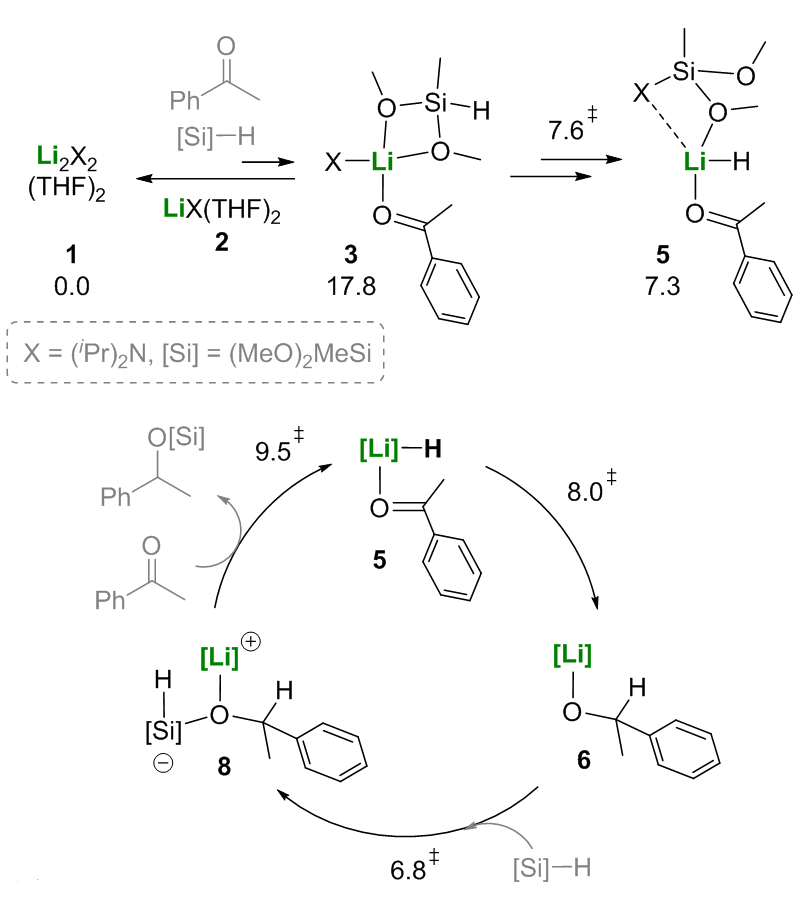
\includegraphics[width=\textwidth]{figures/Ciclo.PNG}
			\end{figure}
		\end{minipage}
		
		\begin{minipage}{0.6\textwidth} 
			\begin{scheme}[H]
				\includegraphics[width=\textwidth]{figures/Energía.PNG}
				\caption{\label{Scheme2} Computed pre-activation step and catalytic cycle, and reaction profile for the hydride-mediated Li-catalysed hydrosilylation of acetophenone. All Gibbs energies are given in THF in kcal mol-1.}
			\end{scheme}
		\end{minipage}
	\end{center}
	
	Figure 1 shows the optimised structures for the key transition states of the pre-activation step. The amide ligand performs a nucleophilic attack to the silicon atom through a reactant-like TS3–4; later, the hydride migrates from silicon to lithium	through the reactant-like TS4-5.
	\\
	We have also computed an alkoxy-silicate-mediated reaction mechanism in the absence of hydride intermediates (Scheme 3). After initial formation of the active species 3, the catalytic cycle continues with amide nucleophilic attack (4), hydrogen transfer (6), and O-Si bond formation to form intermediate 9. Final regeneration of species 3 releases the product. All steps within the cycle present larger activation Gibbs energies	(19–26 kcal mol-1) compared to those in the previous hydride-mediated pathway (7-10 kcal mol-1).
	
	\begin{figure}[H]
		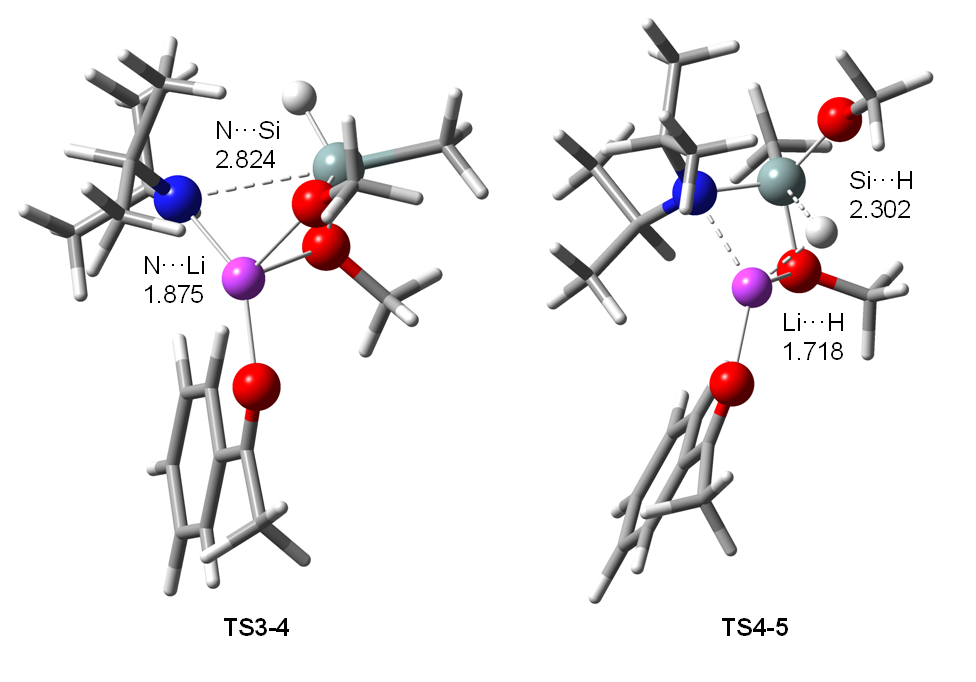
\includegraphics[width=0.5\textwidth]{figures/Nucleophilic attack.PNG}	
		\centering
		\caption{Optimised TS structures for nucleophilic attack (TS3-4) and hydride transfer (TS4-5). All distances in \si{\angstrom}.}
		\label{Figure1}
	\end{figure}	
	
	\begin{scheme}[H]
		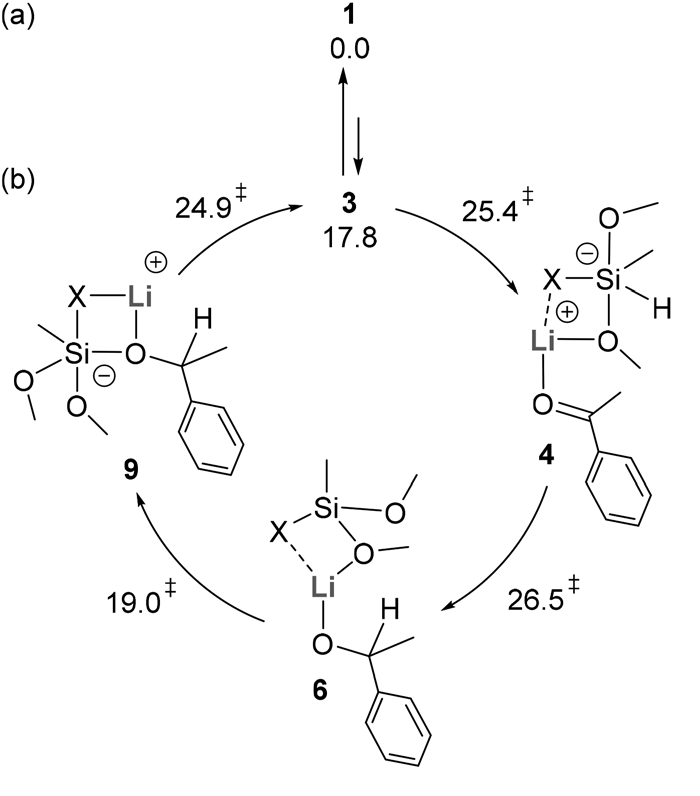
\includegraphics[width=0.4\textwidth]{figures/Cycle.PNG}		
		\centering
		\caption{Computed (a) pre-activation step and (b) catalytic cycle the alkoxy-silicate-mediated Li-catalysed hydrosilylation of acetophenone. All Gibbs energies are given in THF in kcal mol-1.}
		\label{Scheme 3}
	\end{scheme}	
	
	Overall, the computational results suggest a rate-determining activation step to generate the catalytically active species 5, where a great part of the energy toll is related to the initial formation of a monomeric species 3 (Scheme 2a). We then envisage that using deaggregation agents (DAs)17 to displace the equilibrium towards monomeric species would entail a significant	increase in catalytic activity. DAs could also avoid oligomerization of other species such as 5 or 6. In a more general	way, the presence of DAs may favour or stabilise Li species	with lower levels of aggregations. 
	
	It is well documented how the reactivity of organolithium reagents shows significant solvent and co-solvent dependence.18 Most prominently, chelating N and O donor ligands such as pentamethyldiethylenetriamine (PMDTA), tetramethylethylenediamine 	(TMEDA), hexamethylphosphoramide (HMPA), and dimethylpropyleneurea (DMPU) are employed to deaggregate oligomeric s-ock organyls.19,20 Indeed, they can improve product yields, alter product distributions, and increase reaction rates through solvation and chelation of the metallic cations.21 Unfortunately, HMPA is a substance suspected	of carcinogenic potential in humans, and therefore appropriate safety procedures should be followed when handling this reagent in large-scale. 
	
	As a tentative approach to evaluate the impact of DAs on	reactivity, we have included one HMPA molecule during the
	rate-determining formation of the catalytically active species (Scheme 4). In species 1, HMPA displaces one THF; in species
	3, 4, and 5, it displaces the non-participating acetophenone. The computed Gibbs energies indicate that all intermediates
	are stabilised in the presence of HMPA. These results suggest a	better catalytic performance, either by facilitating the deaggregation of Li species (i.e., 17.8 kcal mol-1 from 1 to 3 vs. 12.6 kcal mol-1 from 1-DA to 3-DA) or by increasing the lifetime of key intermediates in solution (i.e., via the formation of 5-DA at 1.3 kcal mol-1). It is important to mention that the higher dielectric constant of HMPA, compared to THF, can have an impact on the computed energies when using continuum solvation models. Assuming that the amount of HMPA added to the solution is rather small (see later experiments),
	we expect similar energies for pure THF and HMPA-THF mixtures at our current level of theory.
	
	\begin{scheme}[H]
		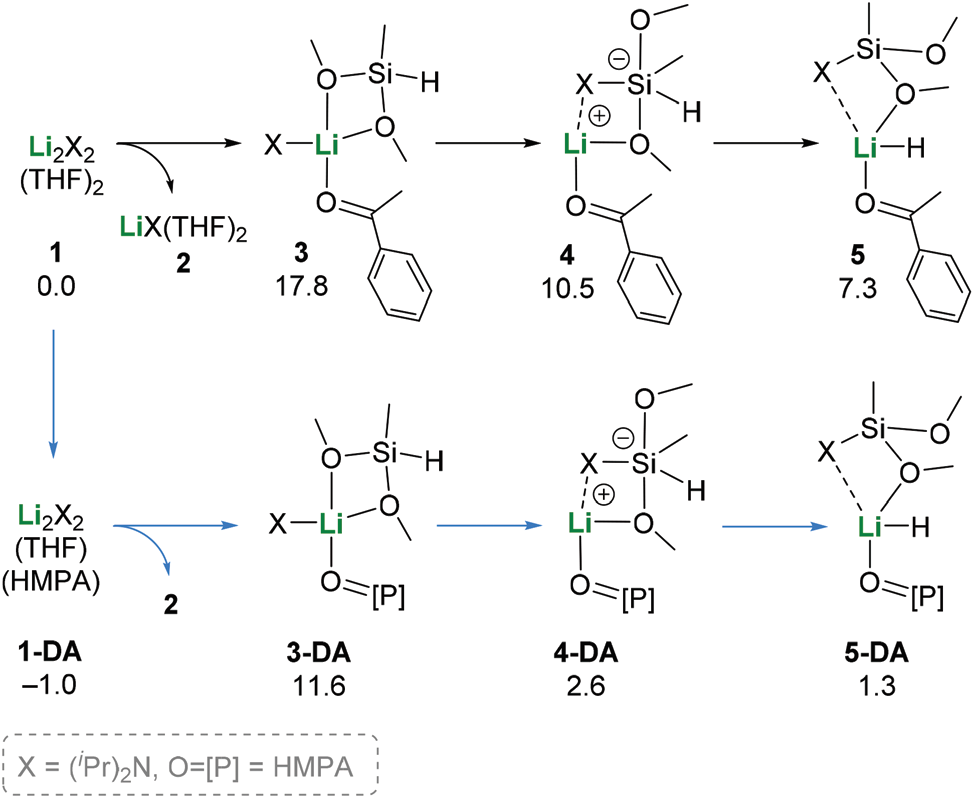
\includegraphics[width=0.7\textwidth]{figures/CompHMPA.PNG}		
		\centering
		\caption{Computed key intermediates in the presence of HMPA. All Gibbs energies are given in THF in kcal mol-1.}
		\label{Scheme4}
	\end{scheme}
	
	To prove this hypothesis on Li-catalysed (0.25\% mol) hydrosilylations, we conducted a series of reactions catalysed by
	commercial amides (lithium diisopropylamide or LDA, lithium bis(trimethylsilyl) amide or LiHMDS, and lithium tetramethylpiperidide or LiTMP) as well as by the anthraquinoid lithium	hydrazone LiAQ,9 each of one in the presence (1.5\% mol, sixfold with respect to the catalyst) and the absence of DAs (Scheme 5 and Table 1). We firstly select HMPA as a representative example due to its commonly usage for this purpose.22 These catalytic runs were monitored via 1H NMR spectroscopy, which allowed us to detect initial rates, culmination steps and conversions (Fig. S1-7). The catalytic outcome remained the same when increasing the excess of HMPA up to 12-fold or 32-fold.
	
	\begin{scheme}[H]
		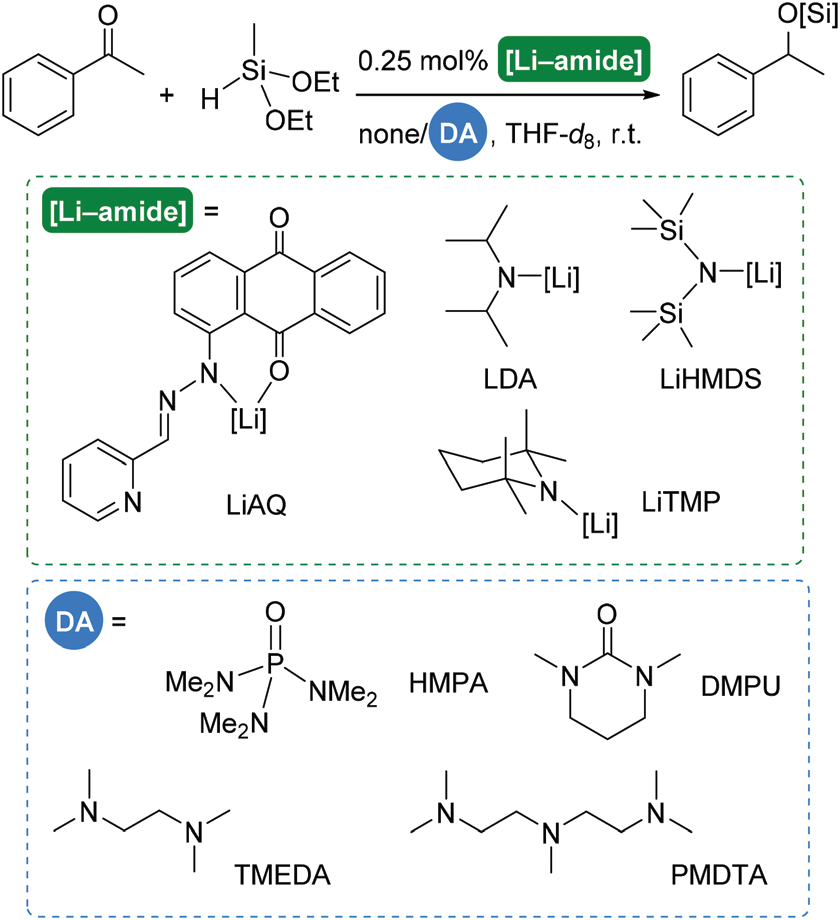
\includegraphics[width=0.6\textwidth]{figures/Reaction.PNG}		
		\centering
		\caption{Reaction conditions: acetophenone (1.0 mmol), (EtO)2MeSiH (1.1 mmol), Li-amide precursor (0.25 mol\%), deaggregation
			agent (none or 1.5 mol\%), THF-d8 (0.5 mL), 294 K.}
		\label{Scheme5}
	\end{scheme}
	
	\begin{table}
		\caption{Turnover frequency (TOF) values obtained at different conversions for the hydrosilylation of acetophenone. LDA, LiHMDS, LiTMP, and LiAQ as catalysts and (EtO)2MeSiH as reducing agent}
		\begin{tabular}{|c|c|c|c}
			\hline
			Entry & Conditions a & TOF 30\%/min-1 & TOF 95\%/min-1 \\
			\hline
			1 & LDA & 11.4 & 2.1 \\
			\hline
			2 & LiAQ & 12.4 & 1.5 \\
			\hline
			3 & LiTMP & 12.2 & 1.4 \\
			\hline
			4 & LiHMDS & 14.7 & 2.2 \\
			\hline
			5 & LDA, HMPA & 45.3 & 19.1 \\
			\hline
			6 & LiAQ, HMPA & 56.4 & 1.9 \\
			\hline
			7 & LiTMP, HMPA & 82.4 & 7.9 \\
			\hline
			8 & LiHMDS, HMPA & 58.2 & 17.4 \\
			\hline
			9 & LiHMDS, DMPU & 27.4 & 2.5 \\
			\hline
			10 & LiHMDS, TMEDA & 28.0 & 2.0 \\
			\hline
			11 & LiHMDS, PMDTA & 18.0 & 2.1 \\
			\hline
		\end{tabular}
	\end{table}
	
	
	As shown by the turnover frequency (TOF) values calculated at two different conversion steps (Table 1) and the kinetic profiles (Fig. S1–7), the reaction rates increased in the presence of catalytic amounts of DA. We observed an enhanced performance	of 4–5 times at 30\% conversion and 8–9 times at 95\% conversion. Neither the catalytic runs in the absence nor the	presence of DA evidenced significant induction periods in their kinetic profiles. In addition, control experiments aimed to rule out the potential catalytic role of the neutral deaggregation agent alone were performed, resulting in absence of
	reaction.
	
	\begin{figure}[H]
		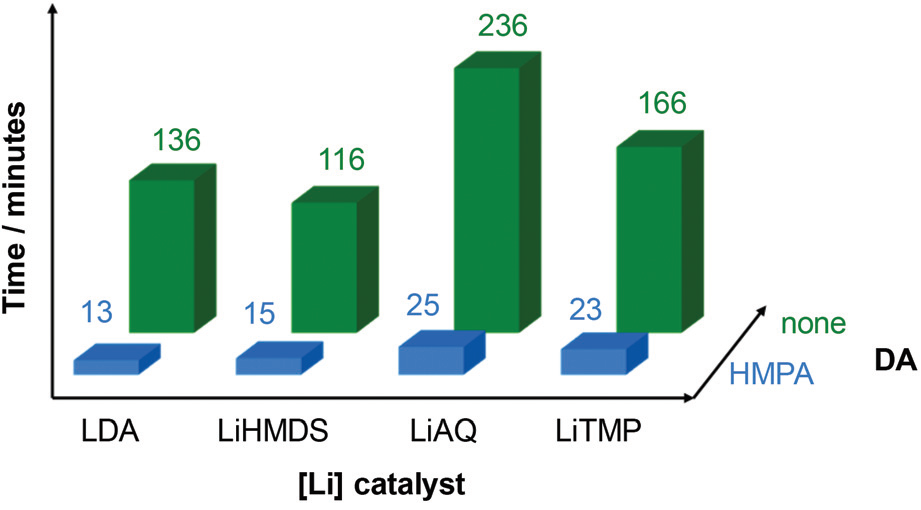
\includegraphics[width=0.6\textwidth]{figures/Bars.PNG}		
		\centering
		\caption{Catalytic hydrosilylation times (in minutes) required to reach 90\% conversion in absence (green bars) and presence (blue bars) of HMPA. All of them used (EtO)2MeSiH as silane at 294 K.}
		\label{Figure2}
	\end{figure}

	Fig. 2 shows the reaction times required to reach 90\% conversion on each catalytic run with (blue) and without (green)	HMPA. In absence of DA, all tested Li-amides showed a similar	behaviour with excellent conversions in times of about 3 h.
	\\The presence of DA evidenced an extraordinary boost, reaching excellent conversions in less than 30 min. In the case of	LDA, the reaction is complete within just 13 min. The accelerating effect of HMPA has been previously noted in s-block20 and lanthanide23 metal catalysis. For instance, Spielmann et al.20a	described a 2.3 acceleration factor in the hydrogenation of
	alkenes with hydrogen after adding a 7.5\% of HMPA with	respect to the main solvent THF. Buch et al.20b described that
	the presence of 3 equiv. of HMPA in the coordination sphere of the calcium catalyst favoured the conversion in the dehydrogenative	silylation of amines and alkynes, thus proving that HMPA played an essential role in these catalytic systems. This synthetic	procedure reproduced an earlier one described by Takaki and	co-workers using ytterbium and samarium analogues bearing HMPA as coordination ligands, although the silylation did not take place when the complexes were prepared in the absence of HMPA.23a,c Similar complexes have also demonstrated their activity in the catalysed hydrosilylation of olefins23b and in the hydrophosphination of conjugated dyenes.23d
	\\As mentioned before, the proposed mechanism involves the	coordination of Li to the alkoxy substituents of the silane	(Scheme 2a). The existence of such intermediates was proven by mixing the LiAQ catalyst and the silane in a J-Young NMR tube. Interestingly, some of the signals in the 1H NMR spectrum of LiAQ were broadened suggesting that averaged signals were detected coming from a fast equilibrium between LiAQ-1 and LiAQ-2 (Scheme 6).
	
	\begin{scheme}[H]
	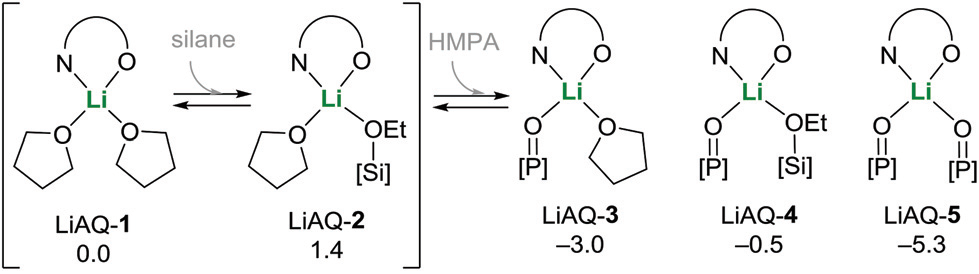
\includegraphics[width=0.8\textwidth]{figures/Equilibria.PNG}		
	\centering
	\caption{Equilibria of LiAQ with silane and HMPA in THF solution unravelled by NMR spectroscopy within the reaction time. Relative Gibbs energies of proposed species are reported in THF in kcal mol-1.}
	\label{Scheme6}
	\end{scheme}

	DFT predicts a Gibbs energy difference of only 1.4 kcal mol-1, in line with the equilibrium observed at the NMR time scale. The signals that underwent significant broadening corresponded to protons in the anthraquinone moiety, while those belonging to the pyridine remained unaltered.9 As expected, when acetophenone is added to this reaction mixture, quantitative formation of product is eventually observed. When HMPA (1.5\% mol) is added to the former reaction mixture, the 1H NMR aromatic pattern (Fig. S9) remains unaltered whatmakes reasonable that a similar mononuclear species may predominate	in THF solution. The 31P NMR spectrum (Fig. S11) shows a relatively broad singlet (W1/2 = 33.8 Hz) located at 24.0 ppm, that is only down-field shifted 0.5 ppm with respect to free HMPA ($\delta$P = 23.5 ppm). Interestingly, the 7Li NMR spectrum at 294 K (Fig. S10) showed two broad signals of W1/2 of ca. 160 Hz each of one located at 1.8 and 1.4 ppm in a ratio 2 : 1, respectively. These data suggest that HMPA coordinates to Li inducing a slower equilibrium which is observable in the	7Li NMR time scale. DFT supports such claim with the exergonic formation of LiAQ-3-5 (Scheme 6). To expand the methodology to other types of DAs, we run the catalytic hydrosilylation reactions in the presence of DMPU, TMEDA, and PMDTA (entries 9-11 in Table 1). Again, the reactions rates increased 2 times in the first period of the	reaction (at ca. 30\% conversion), and with a non-apparent enhancement until the end of the process. That is, whereas the effect of HMPA was maintained during the whole reaction, the behaviour of DMPU, TMEDA, and PMDTA is apparently reduced within the reaction time. This effect may be due to the stronger Lewis base donor ability of HMPA compared to the other additives as well as its high dipolar character.24,25 Same results were found when increasing the concentration of these DAs up to 100 mol\% (Table S1). Current efforts are focused on the design and evaluation of others HMPA-related DAs with less toxicity.26
	
	
% CONCLUSIONS
	\section{Conclusions}
	In this work, we have proposed reaction mechanisms for the Li-catalysed hydrosilylation of ketones using computational methods. Based on these results, we have tested and demonstrated
	experimentally the role of deaggregation agents in catalysis through equilibrium displacement towards active species with lower levels of aggregation, particularly in the presence of
	HMPA where the effect on reaction kinetics is remarkable. We are currently evaluating the impact of these results in other Li-catalysed processes.

% EXPERIMENTAL SECTION
	\section{Experimental section}
	{\bf General procedures of laboratory}
	
	All procedures involving moisture-sensitive components were	performed under an inert atmosphere of dinitrogen, using standard Schlenk techniques or a glovebox. Acetophenone was purified and dried via standard procedures.  Diethoxymethylsilane, hexamethylphosphoramide (HMPA), lithium hexamethyldisylazide (LiHMDS) and lithium tetramethylpiperidine (LiTMP) were purchased from commercial sources and used without further purification. Pentamethyldiethylenetriamine (PMDTA), tetramethylethyl-enediamine (TMEDA) and N,N'-dimethylpropyleneurea (DMPU) were distilled from CaH2 or KOH under reduced pressure. THF was dried in a Solvent Purification System (Innovative Technologies) prior to use. Perdeuterated THF (THF-d8) was purchased from Eurisotop and dried over activated 4 \si{\angstrom} molecular sieves before use. Lithium diisopropylamide (LDA) was prepared from diisopropylamine and n-BuLi
	following standard procedures. Complex LiAQ was prepared as previously described.9 NMR measurements were carried out on
	a Bruker Avance III 500 spectrometer equipped with a TBI (1H/31P/ BB) probehead.
	
	{\bf Experimental procedure for the catalysed hydrosilylation
	reactions monitored by NMR}

	In a glovebox, a stock solution of the catalyst was prepared by	dissolving the corresponding lithium amide (0.0025 mmol) in 1 mL of THF-d8. Then, a NMR sample tube equipped with a J. Young cap was charged with 0.3 mL of THF-d8, (EtO)2MeSiH
	(1.1 mmol, 182 $\mu$L), acetophenone (1 mmol, 118 $\mu$L), and	finally 0.1 mL of the stock solution of lithium amide catalyst (0.0025 mmol). The tube was sealed, shaken manually to	ensure homogeneity and then placed inside the NMR spectrometer, were the sample stayed during the whole set of measurements. For the experiments containing HMPA (0.015 mmol, 2.61 $\mu$L), it was added to the tube right before the catalyst.
	
	{\bf Experimental procedure for the preparation of a sample based on stoichiometric amounts of silane, HMPA and catalyst}
	
	In a J. Young NMR tube, complex LiAQ (0.012 mmol, 9.6 mg) was dissolved in 0.8 mL of THF-d8 and then (EtO)2MeSiH (0.024 mmol, 4 $\mu$L) was added. After 2 hours, a broadening of the signals corresponding to the anthraquinone moiety was
	observed. Then the J. Young tube was taken into the glovebox and HMPA (0.096 mmol, 16.7 $\mu$L) was added. The NMR monitoring was continued for 15 hours without significant changes being observed.
	
	{\bf Computational details}
	
	All calculations were carried out at density functional theory (DFT) level using the M06-2X density functional27 as
	implemented in Gaussian 09.28 Numerical integrations were performed with an ultrafine grid. To model lithium species in
	solution, geometry optimizations were performed in THF solution using the continuum SMD approach and the 6-31G** basis sets for all atoms. Diffuse functions were added for O atoms. The natures of all stationary points were confirmed by computation of vibrational frequencies. Transition	state structures were verified to connect with the corresponding reactants and products by following normal modes associated with their imaginary frequencies. Gibbs energies in	THF were calculated by adding Gibbs energy contributions to	single-point calculations using a larger 6-311++G** basis set. A factor of RT·ln(24.46) was included to take into account the 1 atm to 1 M standard-state Gibbs energy change	(12.33 M for THF). All energies correspond to Gibbs energies at 298 K in THF in kcal mol-1.
	
	Modern DFT methods result from the Hohenberg-Kohn theorem
		\begin{enumerate}
		\item The external potential $V_{ext}$, and hence total energy is a unique functional of the electron density $\rho(r)$
				\begin{align*}
					{\mathrm {Energy}} = \dfrac{\langle\Psi\mid\hat{H}\mid\Psi\rangle}{\langle\Psi\mid\Psi\rangle} \equiv E[\rho]
				\end{align*}
		\item The ground state energy can be obtained variationally, the density that minimizes the total energy is the exact ground state density
				\begin{align*}
					E[\rho] > E[\rho_0], {\mathrm if }\rho \ne \rho_0
				\end{align*}
		\end{enumerate}
	If density is known, then the total energy is:
		\begin{align*}
			E[\rho]=T[\rho]+V_{ne}[\rho] + J[\rho] + E_{nn} + E_{xc}[\rho] 
		\end{align*}
		where 
		\begin{align*}
			E_{nn}[\rho] = \sum_{A>B}\dfrac{Z_AZ_B}{R_{AB}}  \hspace{1cm}&\hspace{1cm}
			V_{ne}[\rho] = \int\rho(r)V_{ext}(r)dr \\
			J[\rho] = \dfrac{1}{2}&\int\dfrac{\rho(r_1)\rho(r_2)}{r_{12}}dr_1dr_2
		\end{align*}

% BIBLIOGRAFÍA	
	\bibliography{proyecto-final}

		
\end{document}